\documentclass[9pt]{article}

\usepackage[utf8]{inputenc}
\usepackage{geometry}
\geometry{
    a4paper,
    total={170mm,257mm},
    left=15mm,
    right=15mm,
    top=20mm,
    bottom=20mm,
}
\usepackage{multicol}
\usepackage[font=small,labelfont=bf]{caption}
\setlength{\columnsep}{0.25cm}
\usepackage[inline]{enumitem}
\usepackage{amssymb}
\usepackage{xcolor}
\usepackage{mathtools} 
\setlength{\parindent}{0em}
\setlength{\parsep}{0em}
\usepackage{tikz}
\setlength{\parskip}{0em}
\usetikzlibrary{decorations.pathmorphing,patterns}
\usepackage[american,cuteinductors]{circuitikz}
\usetikzlibrary{shapes,arrows,circuits,calc,babel}
% Definition of blocks:
\tikzset{%
  block/.style    = {draw, thick, rectangle, minimum height = 3em,
    minimum width = 3em},
  sum/.style      = {draw, circle, node distance = 2cm}, % Adder
  input/.style    = {coordinate}, % Input
  output/.style   = {coordinate} % Output
}
% Defining string as labels of certain blocks.
\newcommand{\suma}{\Large$+$}
\newcommand{\inte}{$\displaystyle \int$}
\newcommand{\derv}{\huge$\frac{d}{dt}$}

\def\mf{\ensuremath\mathbf}
\def\mb{\ensuremath\mathbb}
\def\mc{\ensuremath\mathcal}
\def\lp{\ensuremath\left(}
\def\rp{\ensuremath\right)}
\def\lv{\ensuremath\left\lvert}
\def\rv{\ensuremath\right\rvert}
\def\lV{\ensuremath\left\lVert}
\def\rV{\ensuremath\right\rVert}
\def\lc{\ensuremath\left\{}
\def\rc{\ensuremath\right\}}
\def\ls{\ensuremath\left[}
\def\rs{\ensuremath\right]}
\def\bmx{\ensuremath\begin{bmatrix*}[r]}
\def\emx{\ensuremath\end{bmatrix*}}
\def\bmxc{\ensuremath\begin{bmatrix*}[c]}
\def\emxc{\ensuremath\end{bmatrix*}}
% \def\t{\lp t\rp}
% \def\k{\ls k\rs}

\newcommand{\demoex}[2]{\onslide<#1->\begin{color}{black!60} #2 \end{color}}
\newcommand{\demoexc}[3]{\onslide<#1->\begin{color}{#2} #3 \end{color}}
\newcommand{\anim}[3]{\onslide<#1->{\begin{color}{#2!60} #3 \end{color}}}
\newcommand{\ct}[1]{\lp #1\rp}
\newcommand{\dt}[1]{\ls #1\rs}

\renewcommand{\familydefault}{\sfdefault}

\begin{document}
\begin{center}
\begin{Large}
\textbf{Linear Systems: Least Squares Assignment}
\end{Large}
\end{center}
\vspace{0.2cm}

\begin{multicols}{2}

\begin{enumerate}
    \item The least square approximate solution to  problem $\mf{Ax} = b, \mf{A} \in \mb{R}^{m \times n}$ is obtained by minimizing the following objective fucntion,
    \[ O\lp\mf{x}\rp = \lV\mf{Ax} - \mf{b}\rV^2 = \sum_{i=1}^{m} \lp\tilde{\mf{a}}_i^T\mf{x} - \mf{b}_i\rp^2 \]
    If the the objective function was defined differently, where the different components were given different weights for the different terms, 
    \[ O_w\lp\mf{x}\rp = \sum_{i=1}^{m} w_i\lp\tilde{\mf{a}}_i^T\mf{x} - \mf{b}_i\rp^2 \]
    This is the \textit{weighted least squares}. Find the expression for the approximate solution of the weighted least squares problem.

    \item Consider a matrix $\mf{A} \in \mb{R}^{m \times n}$ with independent columns. There is no matrix $\mf{X}$, such that $\mf{A}\mf{X} = \mf{I}$. Find an expression for the matrix $\mf{X}$, such that $\lV\mf{A}\mf{X} - \mf{I}\rV^2$ is minimum. Hint: Consider the individual columns of $\mf{X}$ and $\mf{I}$.

    \item Consider the following polynomial equation,
    \[ y = \sum_{i=0}^{n} \beta_ix^i, \,\,\,\, x, y, \beta_i \in \mb{R} \]
    This expression is linear in the polynomial coefficients. Fitting a polynomial to data can be done through a linear least square procedure. Conisder a set of measurements $\lc\lp x_l, y_l \rp\rc_{l=1}^{m}$. We are interested in fitting a polynomial that fits this data, such that the difference between the polynomial and data is as low as possible.
    \[ \bmxc y_1\\ y_2\\ \vdots \\ y_m\emxc = \bmxc 1 & x_1 & x_1^2 & \ldots & x_1^n\\ 1 & x_2 & x_2^2 & \ldots & x_2^n\\ \vdots & \vdots & \vdots & \ddots & \vdots\\ 1 & x_m & x_m^2 & \ldots & x_m^n \emxc \bmxc\beta_0 \\ \beta_1 \\ \beta_2 \\ \vdots \\ \beta_n\emxc \]
    \[ \mf{y} = \mf{X}\mf{\beta} \]

    $\mf{X}$ is called the \textit{Vandermonde} matrix. To estimate $\beta$ through a least squares procedure, $\mf{X}$ must have independent columns. Prove that for a set of different $x_i$s the \textit{Vandermonde} matrix has independent columns.

    You are provided with CSV format data file (polyfit.csv) containing data $\lc\lp x_l, y_l \rp\rc_{l=1}^{m}$, to which you are required to fit a polynomial function. The choice of the order of the polynomial is up to you. This can be come from \textit{a priori} knowledge of the system from which data is collected, or it can be decided based on eyeballing the scatter plot between $x_i$ and $y_i$. 

    \begin{enumerate}
        \item \textbf{Data fitting error}: Fit polynomials of orders 0 to 10 to the given data, and for each order determine the data fitting error.
        \[ e_n = \lV\mf{X}\hat{\beta} - \mf{y}\rV \]
        Plot $e_n$ versus the polynomial model order $n$. You should observe the fitting error to monotonically decrease as a function fo $n$. Why is this? Can $e_n$ ever be zero?

        \item \textbf{Model validation}: Even though increasing the polynomial order decreases the data fitting error, this is not always desirable. Given that noise in ubiquitous in all measurements, increasing model order will result in a polynomial that not only fits the general trend in the data, but also the observed measurement noise. Thus, the optimal choice for the model order is determined through a validation procedure, where the data is split into two sets - \textit{training} set and a \textit{testing} set. In order to understand this, you are required to:
        \begin{enumerate}
            \item Split your data $D$ into two sets of size 80\% and 20\%, corresponding to the \textit{training} $D_{train}$ and \textit{testing} $D_{test}$ sets; these percentages are arbitrary. Split you data randomly, such that each data entry is randomly assigned to $D_{train}$ and $D_{test}$.

            \item Fit the polynomial model of a particular order to $D_{train}$. Let the model parameters obtained be $\hat{\beta}$. The validation error for this model is defined as the following.
            \[ e_n^{val} = \lV\mf{X}\hat{\beta} - \mf{y}\rV \]
            where, $\mf{X}$ and $\mf{y}$ comes from the test data set $D_{test}$. Estimate the validation error for different models order 0 to 10, and plot $e_n^{val}$ versus the polynomial model order $n$. How is this plot different from the plot $e_n$ versus $n$? What is the optimal choice for the model order based on the validation procedure?
        \end{enumerate}

        \item \textbf{Regularized data fitting}: Instead of minimzing $\lV\mf{X}\beta - \mf{y}\rV^2$ of the data, now fit a model that minimizes, $\lV\mf{X}\beta - \mf{y}\rV^2 + \lambda\beta^T\beta$, where $\lambda \geq 0$. In this particular case fit the model order to a high value (e.g. 10) and the entire data set $D$. Perform the data ditting procedure for different values of $\lambda$. Plot $\lV\mf{X}\beta - \mf{y}\rV$ verus $\lambda$. Compare the values of $\hat{\beta}$ for the different values of $\lambda$ and compare these to your optimal choice of model parameters from the previous question.
    \end{enumerate}

    \item Consider a time series $\mf{x} = \lc x_0, x_1,\ldots x_{N-1} \rc$ consisting of $N$ data points, where $n$ indicates time index. The time series is corrupted by noise, and we are interested in filtering the time series to obtain a smooth estimate of the the general trend in the time series. This can be posed a problem of estimating a new time series $\hat{\mf{x}}$, such that the difference $\mf{x} - \hat{\mf{x}}$ is minimized and $\hat{\mf{x}}$ is smooth, i.e. the adjacent values of the signal do not change abruptly. 
    \[ O\lp \hat{x} \rp = \sum_{i = 1}^{N} \lp x_i - \hat{x}_i \rp^2 + \lambda \sum_{i = 2}^{N-1} \lp 2 \hat{x}_i - \hat{x}_{i-1} - \hat{x}_{i+1} \rp^2 \]

    If $\mf{x}$ and $\hat{\mf{x}}$ are considered as $N$-vectors, then this can eb written as 
    \[ O\lp \hat{\mf{x}} \rp = \lV \mf{x} - \hat{\mf{x}} \rV^2 + \lambda \lV \mf{D}\hat{\mf{x}} \rV^2 \]

    You are provided with a CSV data file (timeseries.csv) consisting of a time series. Filter this time series by minimizing $O\lp\hat{\mf{x}}\rp$ for different values of $\lambda$. Plot $\mf{x}$ and $\hat{\mf{x}}$ for different values of $\lambda$. What role does $\lambda$ play in the minimzation problem?

    \item Consider the following resistive network, where the horizontal resistors have resistnce of $R_h = 1\Omega$ and the vertical resistors have a resistance of $R_v = 2\Omega$. You goal is to determine a set of currents in the $\mf{i} = \bmx i_1 & i_2 & \ldots & i_{16}\emx^T$, so as to acheive a particular distribution of potentials at the different nodes of the network. Node that we have control only over the currents at the edge nodes, and in the internal nodes the current is zero, i.e. $i_6 = i_7 = i_{10} = i_{11} = 0$.

    \begin{center}
    \begin{circuitikz}[scale=0.8, transform shape]
        \draw (0,0) to[R,*-*] (0,2) to[R,*-*] (0,4) to[R,*-*] (0,6);
        \draw (2,0) to[R,*-*] (2,2) to[R,*-*] (2,4) to[R,*-*] (2,6);
        \draw (4,0) to[R,*-*] (4,2) to[R,*-*] (4,4) to[R,*-*] (4,6);
        \draw (6,0) to[R,*-*] (6,2) to[R,*-*] (6,4) to[R,*-*] (6,6);

        \draw (0,0) to[R,*-*] (2,0) to[R,*-*] (4,0) to[R,*-*] (6,0);
        \draw (0,2) to[R,*-*] (2,2) to[R,*-*] (4,2) to[R,*-*] (6,2);
        \draw (0,4) to[R,*-*] (2,4) to[R,*-*] (4,4) to[R,*-*] (6,4);
        \draw (0,6) to[R,*-*] (2,6) to[R,*-*] (4,6) to[R,*-*] (6,6);

        \draw (-1,7) node[above]{{\Large $i_1$}} to[short, o-] (0,6);
        \draw (2,7) node[above]{{\Large $i_2$}} to[short, o-] (2,6);
        \draw (4,7) node[above]{{\Large $i_3$}} to[short, o-] (4,6);
        \draw (7,7) node[above]{{\Large $i_4$}} to[short, o-] (6,6);

        \draw (7,2) node[right]{{\Large $i_{12}$}} to[short, o-] (6,2);
        \draw (7,4) node[right]{{\Large $i_{5}$}} to[short, o-] (6,4);

        \draw (-1,-1) node[below]{{\Large $i_{16}$}} to[short, o-] (0,0);
        \draw (2,-1) node[below]{{\Large $i_{15}$}} to[short, o-] (2,0);
        \draw (4,-1) node[below]{{\Large $i_{14}$}} to[short, o-] (4,0);
        \draw (7,-1) node[below]{{\Large $i_{13}$}} to[short, o-] (6,0);

        \draw (-1,2) node[left]{{\Large $i_{9}$}} to[short, o-] (0,2);
        \draw (-1,4) node[left]{{\Large $i_{8}$}} to[short, o-] (0,4);

        \draw (0,6) node[below right]{{\large $v_1$}};
        \draw (2,6) node[below right]{{\large $v_2$}};
        \draw (4,6) node[below right]{{\large $v_3$}};
        \draw (6,6) node[below right]{{\large $v_4$}};

        \draw (0,4) node[below right]{{\large $v_8$}};
        \draw (2,4) node[below right]{{\large $v_7$}};
        \draw (4,4) node[below right]{{\large $v_6$}};
        \draw (6,4) node[below right]{{\large $v_5$}};

        \draw (0,2) node[below right]{{\large $v_9$}};
        \draw (2,2) node[below right]{{\large $v_{10}$}};
        \draw (4,2) node[below right]{{\large $v_{11}$}};
        \draw (6,2) node[below right]{{\large $v_{12}$}};

        \draw (0,0) node[below right]{{\large $v_{16}$}};
        \draw (2,0) node[below right]{{\large $v_{15}$}};
        \draw (4,0) node[below right]{{\large $v_{14}$}};
        \draw (6,0) node[above right]{{\large $v_{13}$}};

        \node at (1, 6.5) {$R_h$};
        \node at (-0.6, 5) {$R_v$};
     \end{circuitikz}
     \end{center}

    Let $\mf{v} = \bmx v_1 & v_2 & \ldots & v_{16}\emx$ represent the vector of potential distributions in the network. Then determine $\mf{i}$ such that $\lV\mf{v}_T - \mf{v}\rV^2$ is minimized for the followingdesired potential distribution (Note that the potentias are arragned in a matrix $\mf{V}_{map} = \bmxc 
    v_{1} & v_{2} & v_{3} & v_{4}\\
    v_{8} & v_{7} & v_{6} & v_{5}\\
    v_{9} & v_{10} & v_{11} & v_{12}\\
    v_{16} & v_{15} & v_{14} & v_{13}
    \emxc$
    \begin{enumerate}
        \item $\mf{V}_{map} = \bmxc 
        1 & 2 & 3 & 4\\
        1 & 2 & 3 & 4\\
        1 & 2 & 3 & 4\\
        1 & 2 & 3 & 4
        \emxc $ 
        \item $\mf{V}_{map} = \bmxc 
        2 & 2 & 2 & 2\\
        2 & 1 & 1 & 2\\
        2 & 1 & 1 & 2\\
        2 & 2 & 2 & 2
        \emxc $
        \item $\mf{V}_{map} = \bmxc 
        1 & 1 & 1 & 1\\
        0 & 0 & 0 & 0\\
        0 & 0 & 0 & 0\\
        1 & 1 & 1 & 1
        \emxc $ 
    \end{enumerate}
    for some desired potential distribution $\mf{v}_T$, subject to the constraint $\sum_{k=1}^{16} i_k = 0$.

    \item Trialteration is a process of determining the position $\mf{x} = \bmx x_1 & x_2\emx^T$ of a point $P$ given the distance of the point from a $N$ control points of known locations $\mf{a}_1, \mf{a}_2, \ldots \mf{a}_N$. At any given point in time $n$, we have $N$ different measurements corresponding to the distance of the point $P$ from the $N$ control points, i.e.
    \[ \mf{d}_n = \bmx d_{n1} & d_{n2} & \ldots & d_{nN}\emx^T \]
    where, $d_{ni}^2 = \lV\mf{x}_n - \mf{a}_i\rV_2^2$ for all $1 \leq i \leq N$.
    \begin{center}
    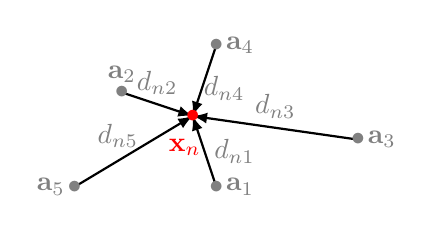
\begin{tikzpicture}[scale=0.6]
        \draw[thick,-latex] (0,0) -- (-0.5, 1.5);
        \node[gray, right] at (-0.25, 0.75) {$d_{n1}$};

        \draw[thick,-latex] (-2,2) -- (-0.5, 1.5);
        \node[gray, above] at (-1.25, 1.75) {$d_{n2}$};

        \draw[thick,-latex] (3,1) -- (-0.5, 1.5);
        \node[gray, above] at (1.25, 1.25) {$d_{n3}$};

        \draw[thick,-latex] (0,3) -- (-0.5, 1.5);
        \node[gray, xshift=0.25cm, yshift=0.2cm] at (-0.25, 1.75) {$d_{n4}$};

        \draw[thick,-latex] (-3,0) -- (-0.5, 1.5);
        \node[gray, xshift=-0.2cm, yshift=0.2cm] at (-1.75, 0.75) {$d_{n5}$};

        \node[gray] at (0,0) {$\bullet$};
        \node[gray, right] at (0,0) {$\mf{a}_1$};
        \node[gray] at (-2,2) {$\bullet$};
        \node[gray, above] at (-2,2) {$\mf{a}_2$};
        \node[gray] at (3,1) {$\bullet$};
        \node[gray, right] at (3,1) {$\mf{a}_3$};
        \node[gray] at (0,3) {$\bullet$};
        \node[gray, right] at (0,3) {$\mf{a}_4$};
        \node[gray] at (-3,0) {$\bullet$};
        \node[gray, left] at (-3,0) {$\mf{a}_5$};
        \node[red] at (-0.5,1.5) {$\bullet$};
        \node[red, xshift=-0.1cm, yshift=-0.1cm] at (-0.5,1) {$\mf{x}_n$};
    \end{tikzpicture}
    \end{center}

    $\mf{x}_n$ are nonlinear functions of the measurements and the control point locations. However, taking the difference between two squared distance measurements $d_j^2$ and $d_i^2$ results in linear equations in the unknown coordinates,
    \[ \lp \mf{a}_i - \mf{a}_j\rp^T\mf{x} = \frac{\lp d_j^2 - \lV\mf{a}_j\rV_2^2 \rp - \lp d_i^2  - \lV\mf{a}_i\rV_2^2 \rp}{2} \]

    Consider the point $P$ that moves with time; $\mf{x}_n \in \mb{R}^{2}$ represents the location of the point at time instant $n$. The distance of this point from a set of 50 different control points is given to you in a CSV data file (trilatdist.csv); the data rows correspond to distance measurements from the different control points at a given point in time, while the colums correpond to the distance of the point from a particular control point for all time. The locations of the 50 control points are available in a separate fileCSV file (trilatctrlpos.csv). Each of these distance measurements is affected by noise. You aim is to use these distance measurements to reconstruct the trajecotry of the point $\mf{x}_n$ as a function of time.
    \begin{enumerate}
        \item What is the minimum number of distance measurements you need to estimate the unknown coordinates of the point $\mf{x}$?
        \item You are provided the actual trajectory of point $P$ in the file trilatactpos.csv. How does you estimate compare with that of the actual trajectory? If we are informed that the point $P$ does not undergo large changes in position between two consecutive time instants $n-1$ and $n$, how would you use this information to improve your estimate?
    \end{enumerate}
\end{enumerate}

\end{multicols}
\end{document}